\documentclass{standalone}
\usepackage{tikz}
\usetikzlibrary{decorations.markings}
\begin{document}
\scalebox{2}{
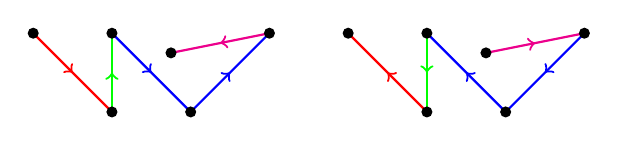
\begin{tikzpicture}
  \begin{scope}[thick,decoration={%
      markings, mark=at position 0.5 with {\arrow{>}}%
    }]
    \coordinate (a1) at (-2,1);%
    \coordinate (a2) at (-1,0);%
    \coordinate (a3) at (-1,1);%
    \coordinate (a4) at (0,0);%
    \coordinate (a5) at (1,1);%
    \coordinate (a6) at (-0.25,0.75);%
    \draw[red,postaction={decorate}] (a1) -- (a2);%
    \draw[green,postaction={decorate}] (a2) -- (a3);%
    \draw[blue,postaction={decorate}] (a3) -- (a4);%
    \draw[blue,postaction={decorate}] (a4) -- (a5);%
    \draw[magenta,postaction={decorate}] (a5) -- (a6);%
    \foreach \i in {1,2,3,4,5,6}%
    \fill (a\i) circle (2pt);%
  \end{scope}
  %
  \begin{scope}[xshift=4cm,thick,decoration={%
      markings, mark=at position 0.5 with {\arrow{>}}%
    }]
    \coordinate (a1) at (-2,1);%
    \coordinate (a2) at (-1,0);%
    \coordinate (a3) at (-1,1);%
    \coordinate (a4) at (0,0);%
    \coordinate (a5) at (1,1);%
    \coordinate (a6) at (-0.25,0.75);%
    \draw[red,postaction={decorate}] (a2) -- (a1);%
    \draw[green,postaction={decorate}] (a3) -- (a2);%
    \draw[blue,postaction={decorate}] (a4) -- (a3);%
    \draw[blue,postaction={decorate}] (a5) -- (a4);%
    \draw[magenta,postaction={decorate}] (a6) -- (a5);%
    \foreach \i in {1,2,3,4,5,6}%
    \fill (a\i) circle (2pt);%
  \end{scope}
\end{tikzpicture}
}
\end{document}
